\documentclass[10pt,conference,compsocconf]{IEEEtran}

\usepackage{hyperref}
\usepackage{graphicx}

\setlength\parindent{0pt}

\begin{document}
\title{Machine Learning Models for the Prediction of Cardiovascular Diseases}

\author{
   Francesco Derme, Pietro Fumagalli, Saransh Chopra\\
  \textit{Machine Learning Course Project 1, EPFL, Switzerland}
}

\maketitle

\begin{abstract}
The present paper addresses the challenge of predicting coronary heart disease from the BRFSS dataset. As the leading global cause of death, developing early-detection models for cardiovascular diseases is critical to improve prevention. We propose and analyze two types of models which correspond to different ways of doing classification: logistic regression and random forests. We show that these models achieve good F1 scores on testing data, providing an effective method for risk assessment. Finally, we experiment with an ensemble model and give recommendations to guide future research.
\end{abstract}

\section{Introduction}
As the mean-age of the global population increases, cardiovascular diseases are an ever-more important threat. Machine learning techniques for the early-detection of these conditions have the potential to save lives by identifying at-risk individuals. We address this challenge by leveraging the health dataset from the Behavioral Risk Factor Surveillance System (BRFSS) \cite{cdc} to build and train binary classification models capable of identifying subjects who are likely to develop a coronary heart disease (MICHD) based on clinical and lifestyle factors. The raw dataset, although vast, lacks quality: it includes missing entries and heterogeneous, unscaled values which necessitate careful pre-processing and feature engineering. The data also suffers from significant class imbalance, with far fewer positive cases than negative ones. We propose two models: logistic regression which models the probability of a subject contracting the disease and then classifies based on a thresholding strategy, and random forests which directly assign a label by following the consensus of an assembly of experts, the trees. We present a comparison of these models, detailing the hyperparameter tuning, cross-validation and threshold strategies aimed at maximizing the F1-score. Finally, we discuss the effectiveness of our models and introduce a novel mixed-approach to be explored further in the future.

\section{Models and Methods}
\label{sec:models-and-methods}

\subsection{Data Pipeline}
The raw BRFSS dataset includes high volumes of missing data as well as features with heterogeneous scales, and special codes of the form \textit{77, 99, 999} used to denote \textit{Refused} or \textit{Not sure} responses. Hence, an extensive manual cleaning of the data is needed to obtain a single, coherent format. We map all special codes to \textit{NaN} and convert features that mix different units of measurement. We then remove features with more than $60\%$ \textit{NaN} entries and split the remaining ones into numerical and categorical and pre-process them differently.\\
For the numerical features, we compute the correlation matrix and find collinear groups, then retain the feature with the fewest \textit{NaN} entries and discard others. An indicator column is created for each numerical feature to hold information about missing data before imputing it. These are needed to ensure that the model can learn from the "missingness" of the data itself. The missing values are then imputed using the median of their respective columns, it acts as a better imputation value than the mean in this case due to its robustness to outliers. Further, all numerical features are standardized to have zero mean and unit variance which is critical for the regularization of the logistic regression model to work as intended. For logistic regression, the numerical features are also polynomially expanded up to degree 2, including squares and a subset of the interaction terms.\\
For the categorical features, \textit{Cramer's V} is used as a measure of categorical association. Features with low predictive power (Cramer's V vs. target lower than 0.1) are removed. We then group highly associated features (Cramer's V higher than 0.8) and, from each group, keep only the single most predictive feature, breaking ties with \textit{NaN} count. For the random forest, ordinal categorical features with many categories are turned into numerical ones to facilitate training. Missing values are imputed using a new category and the final set of cleaned categorical features is one-hot encoded. The whole process is carried out on both train and test sets coherently, without inducing data leakage.

\subsection{Logistic Regression}
A logistic regression is a linear model whose output is converted to a probability by the logistic function. The model is trained using the cross-entropy loss which is smooth and better suited for the task than the F1 evaluation metric. The loss is weighted to account for class imbalance and a plethora of options based on the relative frequencies of the two classes (about 10:1 in the preprocessed dataset) were tested. The loss' gradient is regularized to combat overfitting and the hyperparameter $\lambda$, the regularization strength, is chosen via stratified cross-validation on 5 folds. The training uses the \textit{Adam} \cite{adam} optimizer combined with an exponential-decay learning-rate scheduler. These two techniques, the optimizer and the scheduler, are independent and complementary: the first manages updates of specific weights based on the global rate provided by the second. The training algorithm has a maximum number of epochs (these are "passes" over the whole dataset) which is never reached because training stops if there are no validation-loss improvements in a certain number of epochs (\textit{patience}). Cross validation not only returns the best $\lambda$, but also the ideal number of epochs $\alpha$ to train for. We then perform a final training over $\alpha$ epochs without carving a validation set from the dataset. This does not risk overfitting as we don't give the model enough time to learn the noise in the data. As a threshold is needed to turn probabilities into predictions, we choose the best by evaluating candidates using F1 scores during cross validation. Candidates are chosen by taking quantiles of the predicted probabilities, so that more thresholds are tested in the regions where the model predicts most probabilities (\ref{prob}, \ref{f1}). After careful hyperparameter tuning and several ablation tests, the model achieved 0.429 F1 score on the test set. 

\begin{figure}[t!]
    \centering
    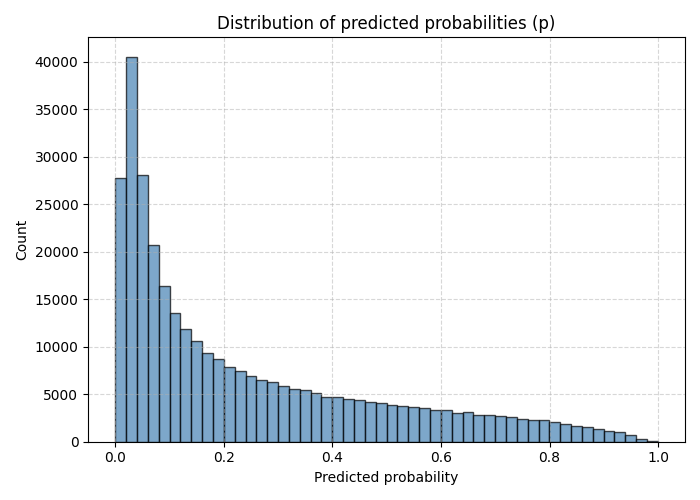
\includegraphics[width=85mm]{probability_distribution.png}
    \label{prob}
\end{figure}

\begin{figure}[t!]
    \centering
    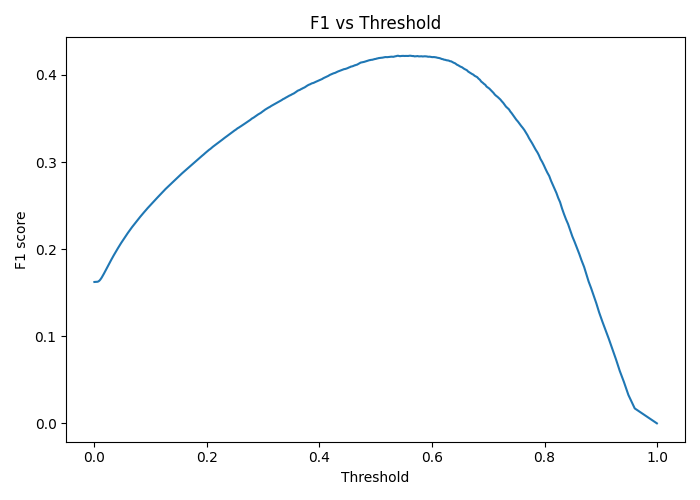
\includegraphics[width=85mm]{f1_vs_threshold.png}
    \label{f1}
\end{figure}

\subsection{Random Forest}
A random forest \cite{rf} is a powerful ensemble method, ideal for non-linear relationships and heterogeneous data. Each decision tree is composed of nodes and each node splits the data by finding the feature and threshold that minimize the \textit{Gini impurity} \cite{gini}, which measures how good a given node is at separating the data. The tree grows recursively until a stopping criterion (like \textit{max depth} or \textit{min samples split}) is met, at which point leaf nodes learn to predict the majority class of the samples they were reached by. At inference time, each sample takes a unique path in any given tree and it's predicted to be part of the class of the leaf it reaches. A random forest is an ensemble of many such decision trees, in particular we used 200. We leveraged two key techniques to reduce variance and prevent overfitting: bagging, which means each tree is trained on a different bootstrap sample (a random sample with replacement) of the training data, and feature randomness, which means that at each split the tree is only allowed to consider a random subset of the total features. We conducted ablation studies focusing on three key components: data sampling, tree regularization, and prediction thresholding. Our experiments demonstrate that balanced bootstrap sampling with a 2:1 ratio of negative to positive class ensures that each tree learns the patterns of the rare positive class. Furthermore, our experiments show that relatively shallow trees (15-20 levels) can produce a better F1 score than deeper trees (25-30 levels) by being less prone to overfitting. We implemented a dedicated threshold tuning function to search a wide range of threshold candidates. Our best random forest achieves its peak F1 score at a threshold of 0.2, which means that 20\% of the trees need to vote positive for a subject to be considered at-risk. After careful hyperparameter tuning and several ablation tests, the model achieved 0.425 F1 score on the test set.

\section{Results and summary}
This paper proposed a logistic regression and a random forest model capable of identifying subjects who are likely to develop a coronary heart disease. The data, although vast, was poor in quality, hence a comprehensive data pipeline was built to clean and standardize it. Logistic regression model with Adam optimizer, exponential-decay learning-rate scheduler, and stratified cross-validation achieved the highest F1 score of 0.429. The random forest model with balanced bootstrap sampling, regularized trees, and threshold tuning lagged behind with an F1 score of 0.425. As part of our experiments, we tested combining both models' predictions into one. Although logistic regression and random forests work on different mathematical principles (the first models probabilities and uses a threshold to take decisions, the second takes a majority vote among trees), it is precisely this heterogeneity that we looked to harness. We experimented with adding the number of positives found by both models, taking averages between the models' predictions, and also tried to account for how confident each model was in its prediction. Although these experiments never achieved a higher F1 score on the test set than 0.429, the idea remains promising and further research is needed to check if predictions from mathematically different models can be merged to create a more accurate prediction. 

\begin{table}[!h]
  \centering
  \begin{tabular}[c]{|l|p{35mm}|l|}
    \hline
    Model&Final model configuration&F1 score on test set\\
    \hline
    Logistic regression&Adam optimizer, exponential-decay learning-rate scheduler, stratified cross-validation&\textbf{0.429}\\
    \hline
    Random forest&Balanced bootstrap sampling, regularized trees, threshold tuning&0.425\\
    \hline
  \end{tabular}
  %\caption{Models, configurations, and F1 scores.}
  \label{tab:results}
\end{table}

\newpage
\bibliographystyle{IEEEtran}
\bibliography{literature}

\end{document}